\section*{Задачник для детей от 15 до 25}
% \author{Трус \and Балбес \and Бывалый}
\begin{figure}[ht!]
    \centering
    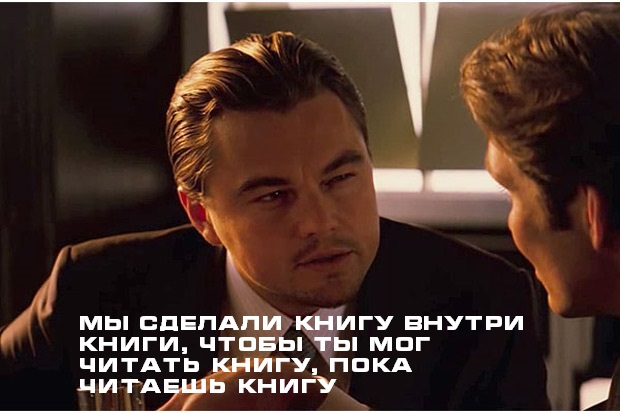
\includegraphics[width=\textwidth]{dicaprio}
\end{figure}

\chapter*{Предисловие}
\addcontentsline{toc}{chapter}{Предисловие}

\begin{flushright}
{\scriptsize С точки зрения математики, люди делятся на два класса: одни предпочитают отнимать и делить, а другие — умножать и складывать.\\
В. И. Арнольд}
\end{flushright}

Привет читатель!\\

Данный сборник хоть и выполнен в стиле уже имеющегося задачника
В.И. Арнольда <<Задачи для детей от 5 до 15 лет>>, но задумывался
авторами как отдельный проект с целью где-то собрать в одном месте
какие-то заинтересовавшие их проблемы и вопросы.\\

Но в ходе работы над сборником было принято решение отдать дань
уважения и попытаться продолжить данный курс книг по воспитанию
культуры мышления.\\

Данная книга поможет скоротать вам скучный вечер и немного расширит ваш кругозор.\\

Задачи были записаны летом 2015 года.\\

Желаем вам приятного времяпреповождения!\\

В память о В. И. Арнольде.\\


\part{Задачи}
    \chapter{Геометрия}
    \begin{problem}
        Определить объём \(n\)-мерной пирамиды, если все рёбра, исходящие из
        одной из её вершин, имеют единичную длину и попарно перпендикулярны.
    \end{problem}
    \begin{problem}
        Определить объём \(n\)-мерного аналога тетраэдра.
    \end{problem}
    \begin{problem}
        Исследовать зависимость отношения объёма гиперсферы к объёму описанного
        около неё гиперкуба от размерности евклидова пространства.
    \end{problem}
    \begin{problem}
        Раскрасить поверхность бутылки Клейна различными цветами так, чтобы
        каждая область определённого цвета граничила со всеми остальными.
        Какое минимальное число цветов необходимо?\\
        \textit{Примечание: точка не является границей двух областей.}
    \end{problem}
    \begin{problem}
        Тор с \(n\) дырками называется тором \(n\)-го рода. Что получится, если
        вывернуть через отверстие тор \(n\)-го рода?
    \end{problem}
    \begin{problem}
        Вычислить \( \int \vec{r} \cdot d\vec{S} \) по следующим
        поверхностям:
        \begin{enumerate}
            \item сфере радиуса \( R \);
            \item эллипсоиду с полуосями \( a \), \( b \) и \( c \);
            \item дикой сферы.
        \end{enumerate}
        \begin{figure}[h]
            \centering
            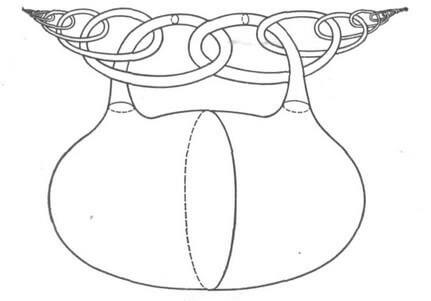
\includegraphics[width=0.5\linewidth]{images/wild-sphere}
            \caption{Та самая дикая сфера}
            \label{fig:wild-sphere}
        \end{figure}
    \end{problem}
    \begin{problem}
        Может ли круг меньшего радиуса содержать в себе круг большего радиуса?
    \end{problem}
    \chapter{Анализ}
    \begin{problem}
        Имеется сферическое однородное облако плазмы, которое покоится в
        начальный момент. Пусть его радиус \( R_0 \), а заряд \( Q_0 \).
        Определить характер его движения и получить зависимость плотности заряда
        от координат и времени \( \rho(\vec{r}, t) \).
    \end{problem}
    \begin{problem}
        Определить закон движения <<солнечного паруса>> (идеально
        отражающего плоского зеркала) площадью \( S \) и массой \(m\) в поле
        тяготения Солнца.
    \end{problem}
    \begin{problem}
        Как будет выглядеть формула Циолковского для фотонной ракеты, двигатель
        которой выполнен в виде параболического зеркала, в фокусе которого
        происходит аннигиляция горючего из вещества и антивещества?
    \end{problem}
    \chapter{Комбинаторика}
    \begin{problem}
        <<Счастливым>> называется билет с 6-значным номером, сумма первых трёх
        цифр которого равна сумме последних трёх\footnote{в Волгограде такие
        билеты называют <<счастливыми по-московски>>; существуют также билеты,
        <<счастливые по-питерски>>}. Сколько всего существует
        <<счастливых>> билетов?
    \end{problem}
    \begin{problem}
        Возможно ли расставить по кругу числа от 1 до 12 так, чтобы для любых 3
        последовательно расположенных чисел \(a\), \(b\) и \(c\) выполнялось
        условие \( b^2 - ac \divisible 13 \)? Если да, то сколько различных
        способов (без учёта начального элемента и направления обхода) существует?
\end{problem}
